%% Document preamble 

\documentclass[12pt]{article}
\usepackage[margin=1in]{geometry}
\usepackage[pdftex]{graphicx}
\usepackage[authoryear,round]{natbib}
\usepackage{amsmath}
\usepackage{amsfonts}
\usepackage{amssymb}


%% title, author, date

\title{EVOLUTIONARY RATE AT THE MOLECULAR LEVEL}

\author{Motoo Kimura \\
NATIONAL INSTITUTE OF GENETICS \\
MISHIMA, JAPAN}


\date{February 17, 1968}

%%% END OF PREAMBLE

%% Main document begins

\begin{document}

\maketitle

\newpage

\abstract{Calculating the rate of evolution in terms of nucleotide substitutions seems to give a value so high that many of the mutations involved must be neutral ones.}

\newpage

\tableofcontents

\listoffigures

\newpage


\section{Premise}

Comparative studies of haemoglobin molecules among different groups of animals suggest that, during the evolutionary history of mammals, amino-acid substitution has taken place roughly at the rate of one amino-acid change in $10^7$ yr for a chain consisting of some 140 amino-acids.  For example, by comparing the $\alpha$ and $\beta$ chains of man with those of horse, pig, cattle and rabbit, the rigure of one amino-acid change in $7 \times 10^6$ yr was obtained \citep{zuckerkandl1965evolving}. This is roughly equivalent to the rate of one amino-acid substitution in $10^7$ yr for a chain consisting of 100 amino-acids.\\


\newpage

\section{Methods}

\citet{hubby1966molecular} estimated that in natural populations of Drosophila pseudoobscura an average of about 12 per cent of loci in each individual is heterozygous.  The corresponding heterozygosity with respect to nucleotide sequence should be much higher. The chemical structure of enzymes used in this study does not seem to be known at present, but in the typical case of esterase-5 the molecular weight was estimated to be about $10^5$ by \citet{narise1966purification}.  In higher organisms, enzymes with molecular weight of this magnitude seem to be common and usually they are ``multimeters'' \citep{fincham1968genetic}. So, if we assume that each of those enzymes comprises on the average some 1,000 amino-acids (corresponding to molecular weight of some 120,000, the mutation rate for the corresponding genetic site (consisting of about 3,000 nucleotide pairs) is \\

$\mu = 3 \times 10^3 \times 5 \times 10^{-10} = 1.5 \times 10^6$\\

per generation.  The entire genome could produce more than a million of such enzymes.\\

\begin{figure}[!ht]
\centering
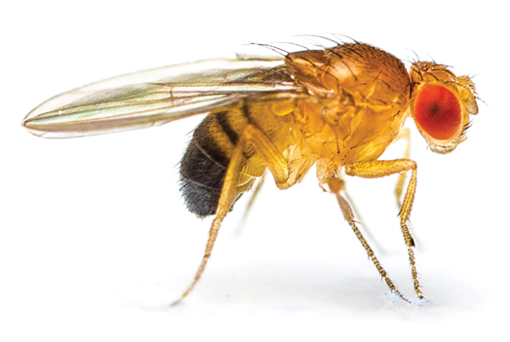
\includegraphics[width=0.6\textwidth]{drosophila}
\caption{A {\it Drosophila pseudoobscura} speciman.}
\end{figure}

\newpage

\section{Conclusions}

Finally, if my chief conclusion is correct, and if the neutral or nearly neutral mutation is being produced in each generation at a much higher rate than has been considered before, then we must recognize the great importance of random genetic drift due to finite population number \citep{wright1931evolution} in forming the genetic structure of biological populations.  The significance of random genetic drift has been deprecated during the past decade.  This attitude has been influenced by the opinion that almost no mutations are neutral, and also that the number of individuals forming a species is usually so large that random sampling of gametes should be negligible in determining the course of evolution, except possibly through the ``founder principle'' \citep{mayr1965animal}. To emphasize the founder principle, but deny the importance of random genetic drift due to finite population number is, in my opinion, rather similar to assuming a great flood to explain the formation of deep valleys but rejecting a gradual but long lasting process of erosion by water as insufficient to produce such a result.


\newpage
%\section{References}

\bibliography{kimura}
\bibliographystyle{plainnat}






\end{document}
